% This is part of the EPRV project 
% Copyright 2022 the authors

% to-do list
% ----------
% - Look for all instances of HOGG, BEDELL, and CITE.
% - Make an acronym command and fix CLRB and all other acronyms.
% - Be sure to discuss SNR in a continuum resolution element, as well as in a pixel.
%.- Make sure that, for any assumption that is explicitly tested, the forthcoming test is mentioned when the assumption is introduced.
% - Are we clear that we exponentiate the model to get the true data expectation?
% - Are we consistent in our use of Doppler shift, radial velocity, and redshift and so on?
% - Are we sensible in our use of first person?
% - Do we address the relationship between our tiny spectral segment and a full spectrograph? Get scalings. Etc.
% - Make sure all figures are explicitly referred to in the text.
% - I believe we are inconsistent with the tense. Always present or always past? Decide and audit / fix. Probably present is better.

\documentclass[modern]{aastex631}
\usepackage[utf8]{inputenc}
\usepackage{amsmath}
\usepackage{amsfonts}

% insanity related to figure frames
\usepackage[framemethod=tikz]{mdframed}
\usetikzlibrary{shadows}
\definecolor{captiongray}{HTML}{555555}
\mdfsetup{%
  innertopmargin=2ex,
  innerbottommargin=1.8ex,
  linecolor=captiongray,
  linewidth=0.5pt,
  roundcorner=5pt,
  shadow=true,
  shadowcolor=black!05,
  shadowsize=4pt
}

% Math macros
\DeclareMathOperator{\CCF}{CCF}
\DeclareMathOperator{\E}{\mathbb{E}}
\newcommand{\dd}{\mathrm{d}}
\newcommand{\given}{\,|\,}
\newcommand{\lao}[1]{\boldsymbol{#1}}
\newcommand{\vy}{\lao{y}}
\newcommand{\vf}{\lao{f}}
\newcommand{\vC}{\lao{C}}
\newcommand{\unit}[1]{\mathrm{#1}}
\newcommand{\m}{\unit{m}}
\newcommand{\cm}{\unit{cm}}
\newcommand{\km}{\unit{km}}
\newcommand{\s}{\unit{s}}
\newcommand{\cmps}{\cm\,\s^{-1}}
\newcommand{\mps}{\m\,\s^{-1}}
\newcommand{\kmps}{\km\,\s^{-1}}

% Text macros
\newcommand{\project}[1]{\textsl{#1}}
\newcommand{\wobble}{\project{wobble}}
\newcommand{\documentname}{\textsl{Article}}
\newcommand{\sectionname}{Section}
\newcommand{\secref}[1]{\sectionname~\ref{#1}}
\newcommand{\figref}[1]{\figurename~\ref{#1}}
\newcommand{\foreign}[1]{\textsl{#1}}

% Hogg typesetting / page layout pedantry
\renewcommand{\twocolumngrid}{}
\setlength{\parindent}{3ex}
\frenchspacing\raggedbottom\sloppy\sloppypar

% headers and date
\renewcommand{\today}{2022 February} % hurt me
\shorttitle{how to measure a radial velocity}
\shortauthors{hogg {\footnotesize\&} bedell}
\begin{document}

\title{How to measure the radial velocity of a star:\\The invariant-spectrum case}
\author[0000-0003-2866-9403]{David W. Hogg}
\affil{The Flatiron Institute, a division of the Simons Foundation}
\affil{Center for Cosmology and Particle Physics, Department of Physics, New York University}

\author[0000-0001-9907-7742]{Megan Bedell}
\affil{The Flatiron Institute, a division of the Simons Foundation}

\begin{abstract}\noindent
    Extremely precise spectroscopic measurements of radial velocity have led to the discovery and characterization of thousands of extra-solar planets.
    Here we ask how to make the best possible radial-velocity measurements, in the sense of information theory.
    That is, how do we make minimum-variance unbiased estimates?
    The answer is: by adopting maximum-likelihood estimates, in the context of a model that is correct in relevant ways.
    Maximum-likelihood estimates can---under certain assumptions---be obtained by maximizing the cross-correlation with a spectral template that accurately represents the true stellar spectrum.
    If there are sufficient spectral measurements of the star, this template can be made empirically, and still produce minimum-variance radial-velocity measurements.
    Cross-correlation with a binary template (which is not in itself a good model for the stellar spectrum) can approach minimum variance if the cross-correlation is followed by a post-processing step in which a smooth model is fit to the cross-correlation function.
    These results justify practices in present-day data pipelines, but also suggest small improvements that might be important.
    HOGG: SENTENCE ABOUT ADDING TELLURIC NOISE, CALIBRATION NOISE, SPECTRAL VARIATIONS.
    The biggest limitation of this analysis is the strong assumption that the star's spectrum does not vary with time.
    This is demonstrably false; we discuss approaches for weakening this assumption.
\end{abstract}

\keywords{foo --- bar} % HOGG

\section{Introduction}\label{sec:intro}

A large fraction of contemporary astrophysics is built on the spectroscopic measurement of radial velocities.
Spectroscopic radial-velocity measurements led to the discovery of the expansion of the Universe (\citealt{hubble}),
dark matter (\citealt{zwicky}, \citealt{rubin}),
and planets around other stars (\citealt{mayor}).
They underpin the empirical basis of almost every branch of astrophysics.
Present-day extreme-precision radial-velocity spectrographs---which now make measurements with better than meter-per-second precision (\citealt{what?})---are responsible for the discovery and characterization of thousands of extra-solar planets.
This project is motivated by the importance of these instruments and their data pipelines in exoplanet science.

In the highest resolution spectrographs ($R\sim 10^5$), a change in velocity of $1\,\mps$ corresponds to a shift in spectral space of $3\times 10^{-4}$ resolution elements, or a shift on the detector of tens of \emph{atomic diameters} (\citealt{zhaophd}).
In this context, how is it possible to measure a radial velocity with better than meter-per-second precision?
The answer to this question is long, but some of the considerations are the following:
The best measurements are made for bright stars, for which a few minutes of exposure time can deliver a spectrum with a signal-to-noise (per resolution element) of hundreds.
These stellar spectra will typically contain tens of thousands of useful absorption lines.
The spectrographs are highly stabilized, and instrumented with excellent calibration sources, often observed simultaneously with the star (\citep{simultaneousreference}, \citep{gascell}).
And, perhaps most importantly, the goal is precision, not accuracy, so the spectrographs need only measure \emph{changes} in the radial velocity at these levels.

Changes in radial velocity are far easier to measure than any individual radial velocity, or even any mean radial velocity, because changes can be measured without a perfectly calibrated theoretical model of the stellar spectrum.
Strictly speaking, there is no stellar-theory-independent measurement of any single radial velocity, because the radial velocity measurement is a measurement of the difference between the observed and true (rest-frame) wavelengths of particular absorption lines, which are produced by non-trivial models of stellar atmospheres.
These atmosphere models involve blended lines, some of which are unidentified, and convective surfaces where there are upwelling and downwelling plasma at different mean temperatures.
That's a mess, and limits the accuracy of the radial-velocity measurement system.
But \emph{changes in time} of the radial velocity of a star can be measured with almost no input of the theory of stellar atmospheres.
This is because the changes from epoch to epoch shift the spectrum straightforwardly.
The shift can be measured even without any model for the true rest-frame spectrum.
If the stellar spectrum doesn't vary---a strong assumption---and some other assumptions about the noise are valid, then changes in radial velocity can be measured with unlimited accuracy, in the sense that the measurements should just get better linearly with the total signal-to-noise in the data set.

Whether you are a Bayesian or a frequentist, you make the best measurements by having a \emph{generative model} for your data.
In both cases, this takes the form of a likelihood function, or a probability density for the data, evaluated at the data, parameterized by a set of parameters including your parameter of interest.
In the Bayesian context, the likelihood function is used to update your beliefs; the posterior pdf is the prior pdf times the likelihood function (and renormalized).
In the frequentist context, the likelihood function can be optimized to produce bound-saturating maximum-likelihood estimates of the parameter of interest.
In what follows, we will concentrate on the latter---information-theoretic bounds on frequentist estimators---but many of the considerations in this \documentname{} will apply also in the Bayesian setting.
In particular, the importance of the assumptions underlying the likelihood function, and the correctness or incorrectness of those assumptions, are equally important in both statistical philosophies.
We will give an example set of assumptions in \secref{sec:assumptions}.

Your radial-velocity measurements are bound-saturating (minimum variance unbiased estimates) when they are maximum-likelihood estimates; we discuss this in \secref{sec:info}.
When the likelihood function is Gaussian, or close, maximum-likelihood estimates can be found by cross-correlation with a spectral template, provided that the spectral template is a good fit to the stellar spectrum; we discuss this in \secref{sec:ccf}.
The original motivation for this \documentname{} was the observation that many radial-velocity data-analysis pipelines perform cross-correlations with a binary mask, which is manifestly \emph{not} a good fit to any stellar spectrum!
Nonetheless, they produce good radial-velocity measurements.
We resolve this paradox in \secref{sec:binary}; the resolution involves the post-processing of the binary-mask cross-correlation function.

Importantly for what follows, the question of having a good template can be made moot, because if the star does not substantially vary, the observations of the star themselves can be used to simultaneously produce the spectral template and the radial-velocity measurements.
We demonstrate this to be true in \secref{sec:templates}.
This is related to the fundamental point, above, that radial-velocity measurements are just measurements of \emph{shifts}; they don't require an \foreign{a priori} model of the spectrum.
We discuss the visualization and checking of empirical models in \secref{sec:testing}, and return to our assumptions in the discussion in \secref{sec:discussion}.

Of course the measurements of radial velocities are not interesting \emph{in themselves}.
In the context relevant to this \documentname, radial velocities are measured in the service of discovering and characterizing extra-solar planetary systems.
These inferences---what you learn about a planetary system from a radial-velocity time series---involve many interesting ideas, including geometry, dynamics, model building, inference, hypothesis testing, and complex nuisances like the Solar System ephemerides.
These topics are all worthy of analysis and discussion, but they are out of scope for this \documentname.

\section{Assumptions}\label{sec:assumptions}

In order to perform any data analysis---and in particular in order to compute anything in information theory---we must make strong assumptions.
These are the assumptions we will make in this project:
\begin{description}
    \item[time-invariant spectrum]
    The most critical (and definitely wrong) assumption is that the intrinsic, rest-frame stellar spectrum does not vary with time.
    All of the standard methods for measuring RVs depend critically on this assumption.
    Weakening this assumption is an extremely important research program for the future of few-$\cmps$ RV measurements, but is beyond the scope of this \documentname, except for abundant discussion.
    \item[multiple epochs]
    We will assume that the star has been observed many times (a number much greater than one). Preferably these observations were taken on different nights, but it is really only the \emph{number} of observations that is required.
    \item[well-calibrated data]
    We will assume that the wavelength grid of the spectrograph is a consistent, correct wavelength grid in the rest frame of the spectrograph.
    We will assume that the measured spectrum is a flux density measurement in consistent flux-density units, normalized (meaning: continuum-normalized) in a consistent way such that the normalization and calibration do not depend on time, nor do they depend on the radial velocity of the star relative to the spectrograph.
    Under these assumptions, the Doppler shift of a spectrum---or really a spectral template---is a pure translation in log wavelength. 
    \item[short exposures]
    We will assume that the exposure times are short relative to the time scales on which the radial velocity relative to the spectrograph changes.
    This isn't precisely true for typical exposures at the present day (minutes), with precisions in the $\mps$ regime; the Earth typically accelerates (relative to the Solar System barycenter) by a few $\mps$ during a 15-minute exposure.
    \item[Gaussian noise]
    Although we will assume that the wavelength grid is precisely calibrated, so there is no significant uncertainty on the pixel wavelengths, we will assume that there is noise in the flux-density measurements, and that the noise draws are Gaussian, zero-mean, and uncorrelated.
    The uncorrelated assumption is easy to relax; we discuss that briefly in \secref{sec:info}.
    In addition to these Gaussian assumptions, we will also make the (stronger) assumption that the variance of the noise distribution is individually known at every pixel.
    We will \emph{not} assume that the noise variance is identical in every pixel; the data will be realistically heteroskedastic.
    \item[manageable tellurics]
    We will assume that any telluric absorption (absorption from the Earth's atmosphere), and also any interstellar absorption, or absorption in the spectrograph, does not interfere in any way with the radial-velocity measurement, either because the tellurics aren't in the spectral range we are analyzing, or they have been masked out or subtracted.
    That is, we will assume that all tellurics are known and accounted for.
    This is not true, of course, and motivates empirical projects like \wobble{} (\citealt{wobble}), to which we will return in \secref{sec:templates}.
    \item[wavelength grid] We will make the strange (but valuable) choice of working not in spectrograph rest-frame wavelength $\lambda$ but instead the natural logarithm of the wavelength, which we will call $x$
    \begin{align}
        x &\equiv \ln\lambda ~.
    \end{align}
    This is a choice, not an assumption, but working in logarithmic wavelength $x$ simplifies the mathematics and notation, because it makes the Doppler shift a linear shift in $x$, and a spectrograph with wavelength-independent resolution $R$ has a line-spread function that is constant-width $1/R$ in $x$.
    More importantly, we will assume that the sampling of the data is good in a Nyquist sense, given the spectrograph resolution; that is, we will assume that the pixel spacing $\Delta x<1/(2\,R)$.
    \item[pure radial Doppler] Related to all of the above, we will treat the RV of the star as a pure shift $\delta x$ in log wavelength $x$.
    The shift $\delta x$ induced by a change $\delta v$ in the radial velocity of the star with respect to the spectrograph is given by
    \begin{align}
        \delta x &= \ln\sqrt{\frac{c + \delta v}{c - \delta v}}\\
        &\approx \frac{\delta v}{c} \mbox{~for~} \delta v \ll c,
    \end{align}
    where $c$ is the speed of light in vacuum.
    This is pretty general, but even this involves some deep assumptions:
    For example, it assumes that there is no plasma or medium along the line of sight that modifies the Doppler formula,
    it assumes (at the interpretation step) that there is no significant transverse component to the Doppler shift,
    and it assumes that the spectrograph has a well-defined velocity (which is not be true for a bench-mounted spectrograph connected to a tracking telescope on a rotating, orbiting planet).
    Related to this, there is a deep assumption that the radial velocity has the same value everywhere in the spectrum.
    This might seem obviously true!
    But in fact it is weakly violated in real data because the throughput of the atmosphere plus spectrograph can be a function of both wavelength and time, and the barycentric contribution to the radial velocity is changing during the exposure (\citealt{berv-lambda}).
\end{description}
Every one of these assumptions is wrong, or badly wrong, or at least questionable.
We will return to them at the end in \secref{sec:sensitivity} and \secref{sec:discussion}.

\section{Information theory}\label{sec:info}

Because data are noisy, there are limits to the precision (and accuracy\footnote{HOGG}) of any measurement that you can make with those data.
The Cram\'er-Rao lower bound (CRLB; \citealt{crlb}) is a quantitative result; it says that the variance of any unbiased estimator $\widehat{\theta}$ of any quantity $\theta$ given noisy data $y$ has a variance greater than or equal to the inverse of the Fisher information $I_\theta$.
The Fisher Information is an expectation of the second derivative of the log-likelihood function with respect to the parameter $\theta$ (\citealt{fisher}); it can only be calculated in the context of a set of assumptions sufficient to deliver a specific likelihood function.
The CLRB is a frequentist bound, because the variance of the estimator, in this case, is the variance obtained in a hypothetical program of repeated experiments (holding everything but the noise draw fixed).
If we make an unbiased measurement $\widehat{\theta}$ of parameter $\theta$ given data $y$ (where this $y$ might be a list or set or vector of observations), that measurement $\widehat{\theta}$ will have expected variance $\sigma_\theta^2$, subject to an inequality:
\begin{align}
    \frac{1}{\sigma_\theta^2} &\leq I_\theta\label{eq:CRLB}\\
    I_\theta &\equiv -\E\left[\frac{\dd^2}{\dd\theta^2}\ln L\right]\label{eq:fisher}\\
    \ln L &\equiv \ln p(y\given\theta)~,
\end{align}
where the first line \eqref{eq:CRLB} expresses the CRLB,
the expectation $\E[\cdot]$ is taken over all possible data sets $y$,
and the likelihood function $L$ is the probability density for the data $y$ given the parameter $\theta$.
Note that since the Fisher information $I_\theta$ involves a second derivative of a dimensionless quantity (a logarithm) with respect to the parameter $\theta$, it has units of inverse-$\theta$-squared, which makes the CRLB consistent in a dimensional sense.

Unbiased estimators that saturate the CRLB are sometimes called efficient estimators.
The simplest way to make an efficient estimator is to optimize the very likelihood function that appears in the definition \eqref{eq:fisher} of the Fisher information.
Maximum-likelihood estimators are popular and successful because they saturate the information-theoretic bound.

Happily, the union of the assumptions listed in \secref{sec:assumptions} is sufficient to deliver a specific likelihood function in the case of interest here.
Therefore we can compute the Fisher information; we have an expectation for the variance of the best possible radial-velocity estimators.
And we can saturate the bounds; we can make radial-velocity measurements that are as good as information theory permits.
In detail, the likelihood function that flows from our assumptions looks like this:
\begin{align}
    \ln L &= -\frac{1}{2}\,\chi^2 - \frac{1}{2}\,\sum_{i=1}^n \ln 2\pi\,\sigma_i^2\label{eq:lnL}\\
    \chi^2 &\equiv \sum_{i=1}^n \frac{[y_i - f(x_i - \delta x)]^2}{\sigma_i^2}\label{eq:chi2}\\
    \widehat{\delta x} &\leftarrow \arg\min_{\delta x} \chi^2 = \arg\max_{\delta x} \ln L\label{eq:argmin}\\
    \frac{1}{\sigma_x^2} = I_x &= \sum_{i=1}^n\frac{1}{\sigma_i^2}\,\left.\frac{\dd f}{\dd x}\right|_{x_i-\widehat{\delta x}}^2\label{eq:ivar}~,
\end{align}
where there are $n$ spectral pixels $i$,
each pixel $i$ is at known log-wavelength $x_i$ and is associated with a normalized spectral flux measurement $y_i$,
that spectral flux measurement has an associated noise variance $\sigma_i^2$,
there is an accurate spectral template $f(x)$,
the Doppler shift is a shift $\delta x$ in the log wavelength,
its estimator or measurement is $\widehat{\delta x}$ with variance $\sigma_x^2$
and
the quadratic form of $\chi^2$ turns the second derivative with respect to $\delta x$ in the definition of the Fisher information into a square of a first derivative of the spectral expectation with respect to log wavelength.
The units of the derivative are spectrum per log wavelength, so when squared and multiplied by the inverse variance of the spectrum, the resulting units of $I_x$ are inverse log wavelength squared.

That is, the best we can do in measuring a Doppler shift, is an inverse variance equal to square of the spectral derivative with respect to Doppler shift, weighted by the inverse variance of the data.
And even this is only possible if the assumptions of \secref{sec:assumptions} hold, and we have a good spectral template $f(x)$.

The expression for $\chi^2$ \eqref{eq:chi2} and for the inverse variance $1/\sigma_x^2$ \eqref{eq:ivar} make the strong assumption that each pixel can be treated independently.
That is, they assume that there are no covariances in the noise distribution from pixel to pixel.
This assumption is often made, but is also often slightly or very wrong, depending on how the spectra are taken, how they are extracted from the 2D CCD image, and how they are continuum-normalized.
If you have a model for the noise covariance (recall our assumption in \secref{sec:assumptions} that the noise is not just Gaussian but that you know the variance of the noise), then you can write a more general expression for $\chi^2$ and the inverse variance:
\begin{align}
    \chi^2 &= [\vy - \vf(\delta x)]^\top\vC^{-1}\,[\vy - \vf(\delta x)]\\
    \frac{1}{\sigma_x^2} &= \left[\frac{\dd\vf}{\dd x}\right]^\top\vC^{-1}\,\left[\frac{\dd\vf}{\dd x}\right]\label{eq:ivar2} ~,
\end{align}
where $\vy$ is an $n$-element column vector containing the pixel values $y_i$,
$\vf(\delta x)$ is an $n$-element column vector containing the template values $f(x_i-\delta x)$,
$\vC$ is an $n\times n$ covariance matrix containing the pixel noise variances on the diagonal and the covariances in the non-diagonal elements,
and $\dd\vf/\dd x$ is the derivative of $\vf$ with respect to the $\delta x$ argument.

These expressions \eqref{eq:ivar} and \eqref{eq:ivar2} for the inverse variance $1/\sigma_x^2$ are extremely simple, but also extremely important for experimental design.
They deliver---implicitly---expectations for (best possible) radial-velocity precision as a function of stellar spectral type, spectrograph resolution, spectral coverage, and signal-to-noise, because these inputs affect the expectations for the template $f(x)$, the noise variances $\sigma_i^2$, and the number of pixels $n$.
These expressions are not new; many related expressions appear in the literature:
HOGG: How are these uncertainty formulae related to formulae in the literature? HOGG: MOVE HERE FROM THE EPRV DOC.

\section{Toy data}\label{sec:data}

In order to test the maximum-likelihood estimator and the estimators to follow, we build a sandbox of completely fake data with known properties, obeying our assumptions.
\figref{fig:data} shows a few example spectra generated from our model.
The model spectra are made with an exactly unit continuum and a set of discrete absorption lines of varying equivalent widths.
The lines are drawn from a uniform Poisson process in the long-wavelength $x$ domain.
Their equivalent widths are drawn from a power-law distribution function.
The spectrograph line-spread function is set to be a Gaussian in the log-wavelength $x$ space, with a standard deviation $\sigma_x=1/R$, where $R=135\,000$ is the spectrograph resolution.
Technically the Gaussian line-spread function is used to generate the logarithm of the flux, which is then exponentiated to deliver the pixel flux expectations.
BEDELL SHOULD WE PUT AN EQUATION HERE, OR IS THIS EXPONENTIATION POINT CLEAR?
The noise on the continuum-normalized spectral pixel values is Gaussian with zero mean and variance proportional to the continuum-normalized spectral expectation (true intensity).
This noise is explicitly white; it is designed to model photon or shot noise.
The noise variance model is normalized to hit a particular signal-to-noise ratio (SNR) in the continuum (that is, at a continuum-normalized flux $y=1$); typically we set this SNR to 100 (per pixel).
The true Doppler shifts $\delta x\equiv\ln\sqrt{(c+v)/(c-v)}\approx v/c$ for the different spectra are generated by a pure sinusoid of the epoch number with an amplitude of $1\times10^{-4}$, corresponding to something like barycentric variation.
We included no telluric absorption in these toy data.
Example spectra are shown in \figref{fig:data} and \figref{fig:datazoom}.

\begin{figure}[tp]
  \begin{mdframed}
    \begin{center}
    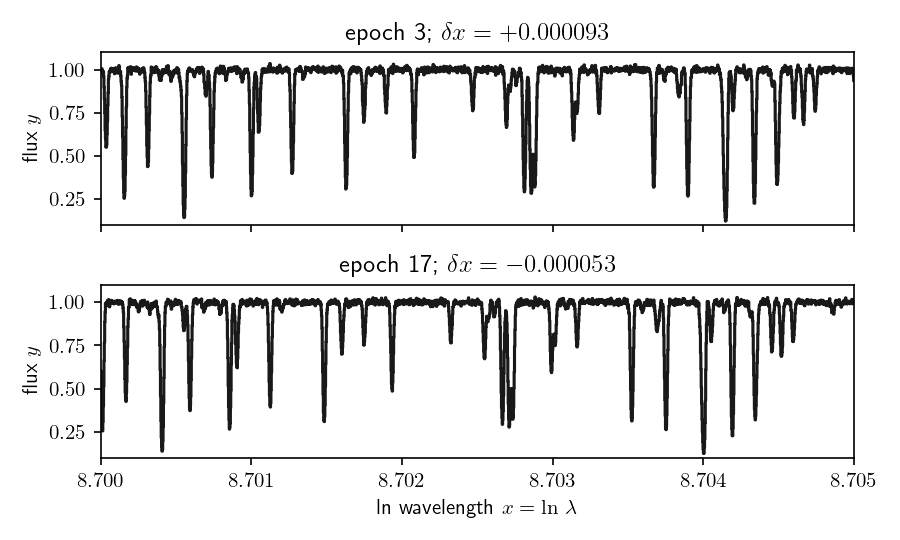
\includegraphics[width=\textwidth]{../notebook/data.png}
    \end{center}
    \caption{Two example toy-data spectra, generated according to the rules described in the main text.
    At each epoch the true spectrum has the same overall shape; the only differences from epoch to epoch are from Doppler-shift changes and shot noise.\label{fig:data}}
  \end{mdframed}
\end{figure}
\begin{figure}[tp]
  \begin{mdframed}
    \begin{center}
    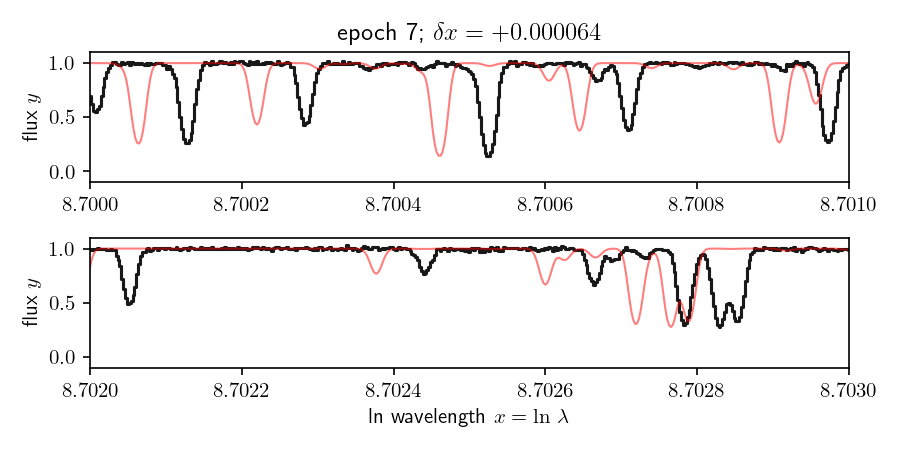
\includegraphics[width=\textwidth]{../notebook/datazoom.png}
    \end{center}
    \caption{A zoom in on one of the toy-data spectra. Shown are both the data (dark black step function) and the true spectral model (thin red smooth line). The data for this epoch is Doppler shifted relative to the model, which is at zero Doppler shift.\label{fig:datazoom}}
  \end{mdframed}
\end{figure}

The toy-data assumptions are unrealistic for an entire extracted spectrum from a present-day spectrograph!
But they are close to appropriate for certain intervals or small segments of spectrum extracted from a high-resolution spectrograph, such as \project{EXPRES} (\citealt{express}):
In small spectral segments, the noise variance (for a bright star) is proportional to the flux, the continuum level is not a strong function of wavelength, the spectrograph resolution is well defined, and the line-spread function is stable.
And indeed, our toy-data simulations span only a small spectral segment.
Importantly, with these toy-data assumptions, we can generate toy data, compute information-theoretic bounds, and test different kinds of radial-velocity estimators.

One detail about our these toy data is that although when we generate the noise we use a variance that depends on the true flux expectation, the observer of these data never gets to see that expectation directly.
For this reason, we produce two different noise variance estimates at every pixel:
One is the true noise variance that is related to the true flux expectation and that was used to generate the noise in that pixel.
The other is an empirical noise variance estimate that is based on the observed (noisy) flux in that pixel.
These two noise variances are very similar except for the faintest pixels---that is, the pixels in the centers of strong absorption lines.
In what follows, we use the true noise variances to estimate the information-theoretic bounds.
We use the empirical noise variances in the log-likelihood function (or chi-squared function $\chi^2$) that is used to produce the maximum-likelihood radial-velocity estimates.

\figref{fig:mlrvs} shows the true radial velocities for the XXX epochs of toy data, the maximum-likelihood radial velocities found by minimizing $\chi^2$ \eqref{eq:chi2}, the residuals, and the information-theoretic (Cram\'er--Rao) bound \eqref{eq:CRLB} derived from the inverse of the Fisher information \eqref{eq:fisher}.
In detail, to obtain these radial-velocity estimates the $\chi^2$ function made use of a stellar template, and here we used the exactly correct template; we used the template that was used to generate the toy data in the first place.
This figure shows, as expected, that with this use of a perfect template, the minimum-$\chi^2$ radial-velocity estimates, which are maximum-likelihood estimates, saturate the information-theoretic bound.

\begin{figure}[tp]
  \begin{mdframed}
    \begin{center}
    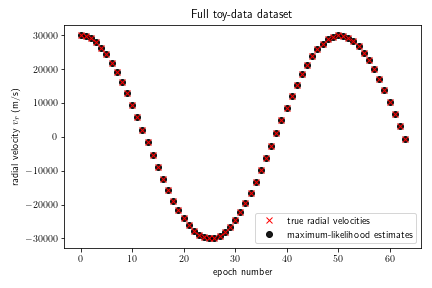
\includegraphics[width=\textwidth]{../notebook/full.png}
    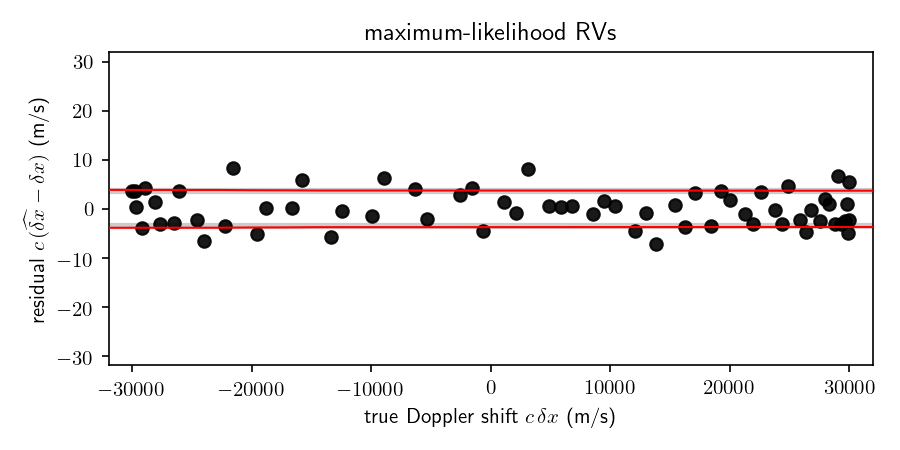
\includegraphics[width=\textwidth]{../notebook/mlrvs.png}
    \end{center}
    \caption{Demonstration that maximum-likelihood estimates saturate the information-theoretic bound.
    The top panel shows both the true doppler shifts for the 64 epochs of toy data and the maximum-likelihood estimates.
    The bottom panel shows the residuals (estimate minus true) as a function of true doppler shift.
    In the bottom panel, the thin red lines indicate the Cram\'er--Rao lower bound on the root-variance (the square-root of the inverse of the Fisher information), and the thick grey lines indicate the empirical central 68-percent region (the empirical one-sigma region).
    The fact that the thin red lines overlap the thick grey lines shows that the maximum-likelihood estimates saturate the information-theoretic bound, as expected.\label{fig:mlrvs}}
  \end{mdframed}
\end{figure}

HOGG: Maybe show that the wrong template (like missing some lines) gives less-good RVs?? Or move this to \secref{sec:sensitivity}??

\section{Cross-correlation}\label{sec:ccf}

Most data-analysis pipelines associated with radial-velocity spectrographs do not explicitly optimize a likelihood function to obtain the radial velocities; nor do they explicitly minimize any kind of chi-squared expression.
Instead they optimize a cross-correlation between the data and a template spectrum.
And yet they deliver excellent radial velocities in general (CITE?).
How is this possible?
It turns out that, under a restrictive set of assumptions, the optimization of a cross-correlation is identical to the optimization of a likelihood function.
Here is the argument:

The estimate $\widehat{\delta x}$ in \eqref{eq:argmin} is a minimum of a $\chi^2$ expression \eqref{eq:chi2}.
The square of the difference in the $\chi^2$ can be expanded as follows
\begin{align}\label{eq:chi2ccf}
    \chi^2 &= \underbrace{\sum_{i=1}^n \frac{y_i^2}{\sigma_i^2}}_{\text{constant}}
         - 2\,\underbrace{\sum_{i=1}^n \frac{y_i\,f(x_i - \delta x)}{\sigma_i^2}}_{\text{like a cross-correlation}}
         +    \underbrace{\sum_{i=1}^n \frac{[f(x_i - \delta x)]^2}{\sigma_i^2}}_{\text{can be made constant}} ~,
\end{align}
where the first term is a constant that doesn't depend on $\delta x$,
the second term is a kind of inverse-variance-weighted cross-correlation between the data $y$ and the template $f(x)$,
and the third term is very close to constant as $\delta x$ varies (and can be made to be exactly constant by suitably normalizing $f(x-\delta x)$).
Thus minimization of a $\chi^2$ (or maximization of a Gaussian likelihood function) is nearly equivalent to maximization of a cross-correlation.
In the covariant-noise case, the cross-correlation becomes something like
\begin{align}
    \sum_{i=1}^n \frac{y_i\,f(x_i - \delta x)}{\sigma_i^2} &\rightarrow \vy^\top\vC^{-1}\,\vf(\delta x)\label{eq:wccf} ~,
\end{align}
but the story is the same---that is, that $\chi^2$ minimization is equivalent to cross-correlation maximization.
Technically a cross-correlation function is defined by an integral, not a sum!
These are the same when the argument of the sum is weighted by the a pixel measure (typically a pixel width) and the pixel measures  go to zero.
The terms in \eqref{eq:wccf} constitute precisely a cross-correlation with an inverse-variance measure in the $x$ space, in the limit that the pixel spacing is tiny.

In the expansion \eqref{eq:chi2ccf}, there are three terms, one is a constant (doesn't depend on the Doppler shift $\delta x$), and one is marked ``can be made constant''.
It turns out that for precise radial-velocity measurement, it is essential that this term be made constant.
The reason it isn't precisely constant under uncontrolled conditions is that as the Doppler shift changes, some absorption lines at the edges of the spectral range enter and leave the domain.
These change slightly the auto-correlation of the template $f(x)$ with itself, when this auto-correlation is restricted (as it is) to the domain of the observed data segment.
Thus it is imperative that the template be renormalized at every Doppler shift by a normalization that looks like this:
\begin{align}
    f(x_i-\delta x) &\leftarrow f(x_i-\delta x)\,\left[\sum_{i=1}^n \frac{[f(x_i-\delta x)]^2}{\sigma_i^2}\right]^{-1/2} ~.
\end{align}
With this Doppler-shift-dependent normalization, the auto-correlation term in the expansion \eqref{eq:chi2ccf} becomes precisely constant with $\delta x$.
This might seem like a detail, but in our toy-data example, failure to renormalize in this manner introduces structured scatter in the radial-velocity estimates far in excess of the information-theoretic bound.

Many data pipelines do a simple unweighted cross-correlation, not weighted by the inverse pixel variances $1/\sigma_i^2$ (nor the inverse covariance matrix $\vC^{-1}$).
Technically maximization of the simple unweighted cross-correlation function is not equivalent, but for much of the spectrum, it won't be very different, because much of the spectrum has uncertainties that lie in a reasonably low dynamic-range band, for the most part.
And besides, in a typical present-day high-resolution spectrograph, the cross-correlation function is an average over hundreds of thousands of pixels, so local variations in the pixel variances aren't extremely important to the final answer, especially if very noisy parts of the spectrum have been censored or masked out.

In terms of detailed implementation, one interesting and perhaps surprising fact is that it is not necessary to do very fine steps in the Doppler shift $\delta x$ when numerically optimizing this cross-correlation.
The reason is that if the data are taken with a spectrograph with well-defined resolution $R$, there can't be sharp features in the cross-correlation function at scales $\Delta(\delta x)<1/R$.
The Doppler shift $\delta x$ can be scanned on a grid that is, say $1/(3R)$ and then the 3 pixels in the empirical cross-correlation peak can be fit with a parabola; the optimal estimate $\widehat{\delta x}$ of the Doppler shift $\delta x$ is the maximum of that parabola.
This is illustrated in \figref{fig:ccf}.

\begin{figure}[tp]
  \begin{mdframed}
    \begin{center}
    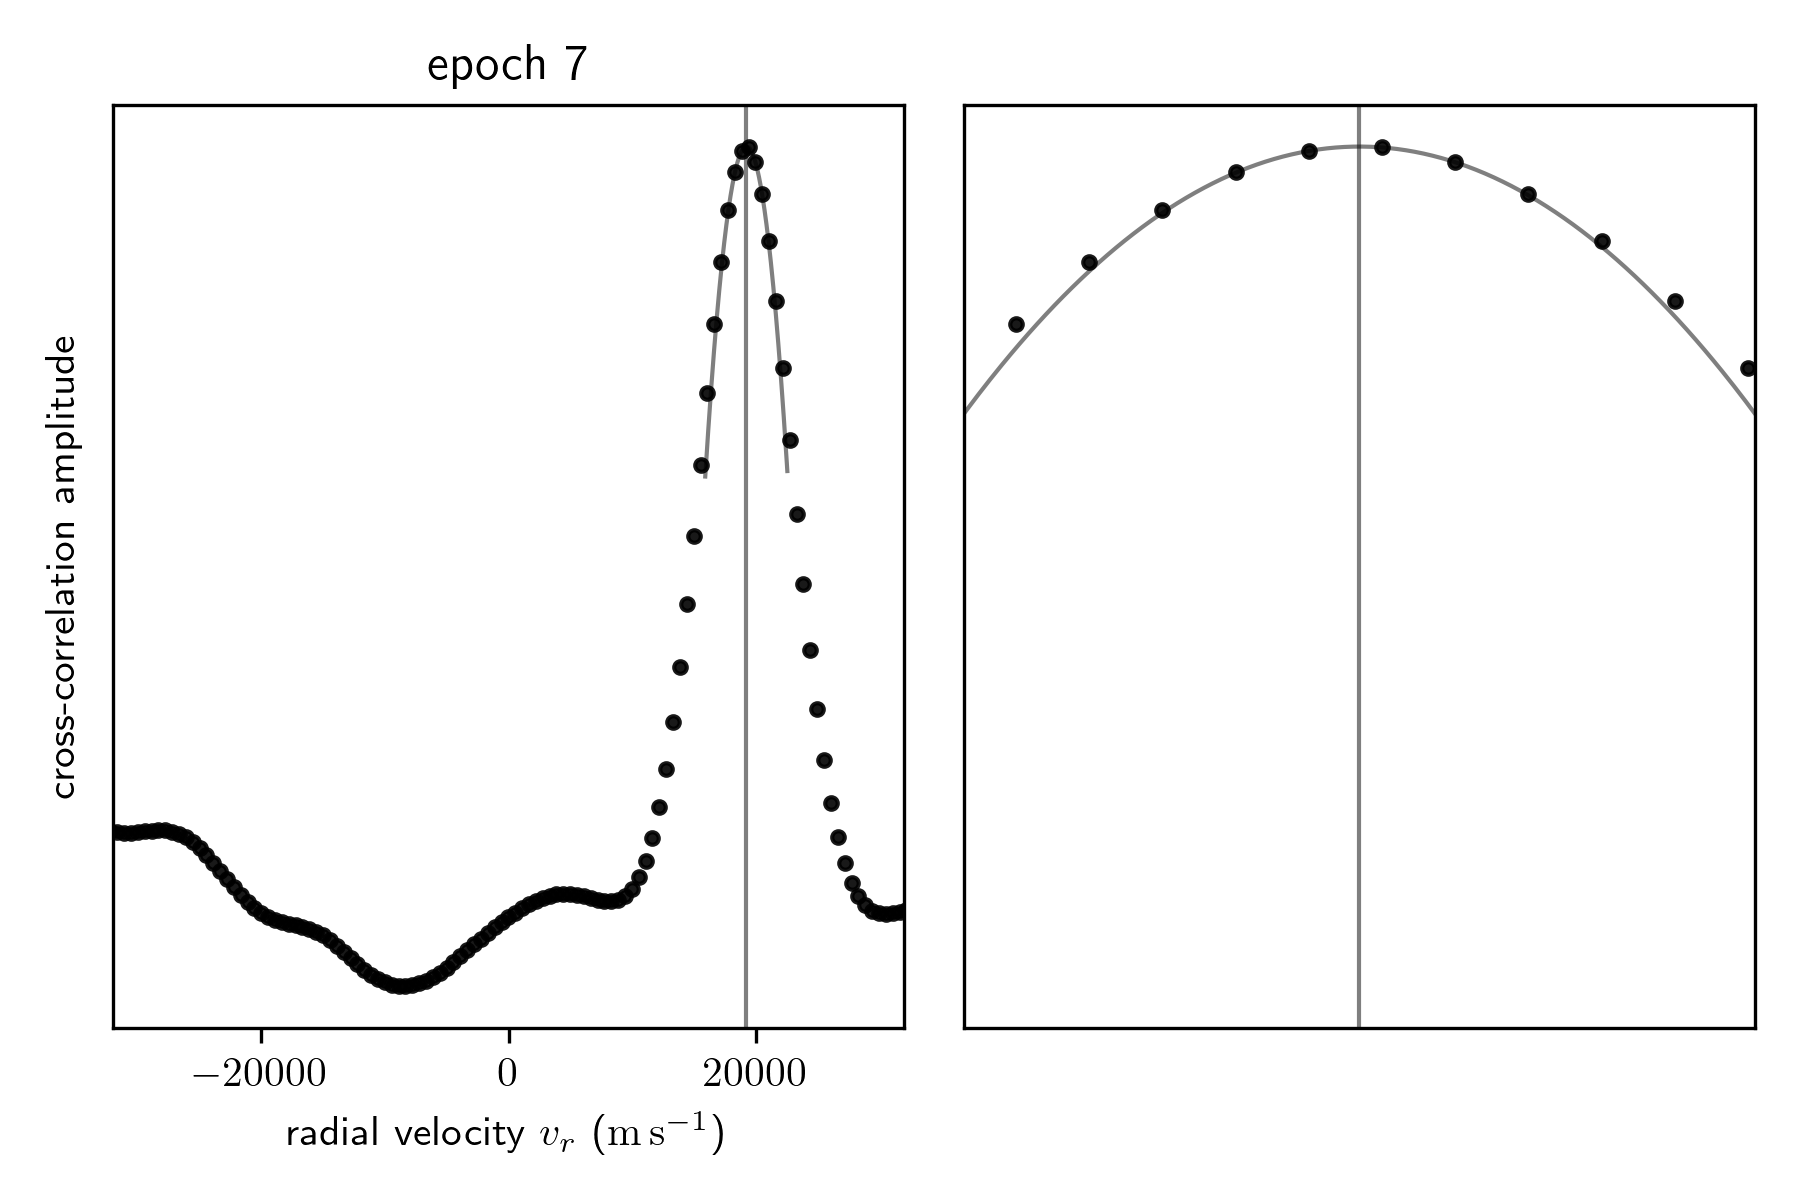
\includegraphics[width=\textwidth]{../notebook/ccf.png}
    \end{center}
    \caption{Optimizing a function with the parabola trick. The left panel shows the cross-correlation amplitude (data cross-correlated with a correct template spectrum) measured at a discrete set of Doppler shifts. The right panel shows a zoom in on the peak. The smooth parabola is fit to the three peak values of the cross-correlation function, and the vertical line shows the optimum of that parabola.\label{fig:ccf}}
  \end{mdframed}
\end{figure}

The cross-correlation radial-velocity measurement precision on the full toy-data dataset is shown in \figref{fig:ccfrvs}.
As expected, these radial-velocity estimates also saturate the information-theoretic bound.

\begin{figure}[tp]
  \begin{mdframed}
    \begin{center}
    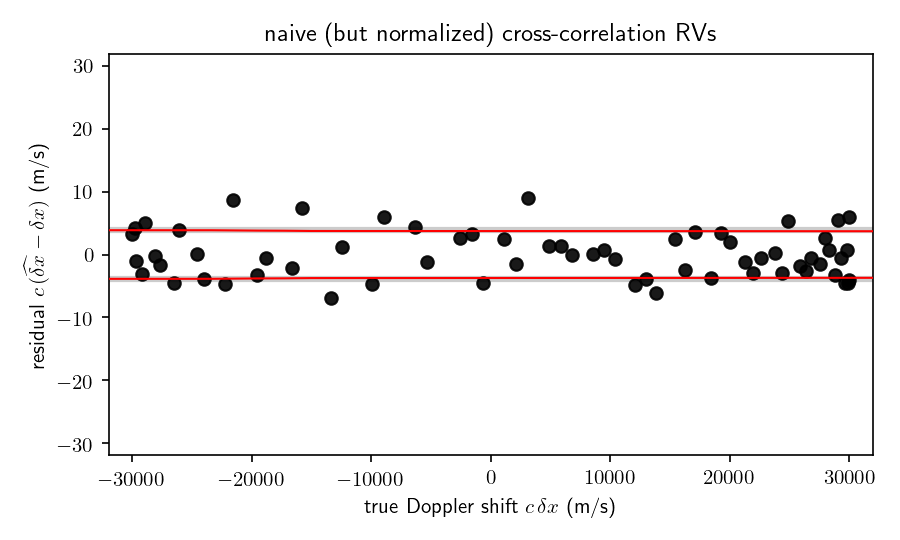
\includegraphics[width=\textwidth]{../notebook/ccfrvs.png}
    \end{center}
    \caption{Same as the bottom panel of \figref{fig:mlrvs}, but for the cross-correlation Doppler-shift estimates. The coincidence of the thin red and thick grey lines shows that the cross-correlation estimates saturate the information-theoretic bound.\label{fig:ccfrvs}}
  \end{mdframed}
\end{figure}

For both the cross-correlation radial-velocities in this \sectionname{} (\figref{fig:ccfrvs}) and the maximum-likelihood radial-velocities shown in \secref{sec:data} (\figref{fig:mlrvs}), it was essential that the template spectrum $f(x)$ be accurate, or accurately represent our expectation for the spectrum.
When the template spectrum does not look like the true spectrum, both biases and additional variance are introduced.
A full description of this is out of scope, but we show one particular example below in \secref{sec:binary} (\figref{fig:wrongbccfrvs}).

\section{Binary mask magic}\label{sec:binary}

In this \sectionname{} we discuss a technical matter relevant to present-day radial-velocity pipelines.
This point is not important to our main information-theory thread, but is relevant to understand why present-day pipelines work well.

We demonstrated, above, that maximum-likelihood or cross-correlation with a good spectral template leads to information-theoretic optimal estimates of radial velocity.
That's important.
However, most present-day operating instrument pipelines (CITE) in fact the extracted spectrum is instead cross-correlated with a \emph{binary mask}.
This is a function that is unity in some wavelength regions, and zero in most of the rest, typically unity in significant stellar absorption lines and zero outside the lines, or in the vicinity of strong telluric absorption.
There is no way that the cross-correlation with this template can directly deliver radial velocities that saturate any bounds!
And yet pipelines \emph{do} produce excellent estimates of radial velocity.

What gives?
First of all, because the binary mask, in some sense, indicates the \emph{negative} of the absorption, the cross-correlation is more-or-less \emph{minimized} at the correct radial velocity, not maximized.
Second of all, the way the cross-correlation is used, in these pipelines, is not that it is directly minimized, but instead the dip in the cross-correlation function is \emph{fit with a smooth model} (usually an inverted Gaussian function).
The radial-velocity measurement is then derived from the offset of the best-fit Gaussian to the binary-mask cross-correlation function.
In a miracle worthy of the name, this procedure is functionally equivalent to convolving the binary mask with a Gaussian---thus making a reasonably good template for the spectrum---and then optimizing the cross-correlation of the data with that good (no longer binary) template.
In what follows, we demonstrate this quantitatively.

Imagine that you have a binary mask function $\beta(x)$ with the beautiful property that if you smooth it with some smooth line-spread function $\psi(x-x')$ it becomes a reasonable model template $y(x)$ for the deviation of the spectrum from the continuum.
Think of the binary mask as being (effectively) an absorption line list, with the width of each binary line in the binary mask corresponding to the equivalent width the line has in the spectrum.
Then convolution with a model $\psi(x-x')$ of the line-spread function will give a model for the finite-resolution spectrum.
That is, imagine that we have a binary mask $\beta(x)$ and kernel function $\psi(x-x')$ such that
\begin{align}
    y(x) &= 1 - \int\beta(x')\,\psi(x-x')\,\dd x' ~,
\end{align}
where $y(x)$ is now a good spectral template, and the $1$ represents the continuum level of that template.
Now pixelize the binary mask, the line-spread function, and the data onto an extremely fine pixel grid.
The convolution becomes
\begin{align}
    f_i &= 1 + \sum_{i'=-k}^k \beta_{i-i'}\,\psi_{i'} ~.
\end{align}
Now the cross-correlation function of the data with this numerically constructed template $f$ can be written as a cross-correlation of the data with the binary mask $b$, subsequently cross-correlated with the the kernel $\psi$.
This, in turn, will be optimized at the same place as a fit of the kernel $\psi$ to the cross-correlation between the data and the binary mask.
In equations (HOGG SAYS: I THINK THERE'S a sign error here):
\begin{align}
    \CCF(\delta; f) &= \sum_{i=1}^n \frac{y_i}{\sigma_i^2}\,\sum_{i'=-k}^k \beta_{i-\delta-i'}\,\psi_{i'} + \text{const}\\
    &= \sum_{i'=-k}^k \CCF(\delta+i';\beta)\,\psi_{i'} + \text{const}\\
    &= -\frac{1}{2}\sum_{i'=-k}^k [\CCF(\delta+i';\beta) - \psi_{i'}]^2 - \text{const}\mbox{~(s.t. conds.)}\\
    \arg\max_{\delta} \CCF(\delta; f) &= \arg\min_{\delta} \sum_{i'=-k}^k [\CCF(\delta+i';\beta) - \psi_{i'}]^2 ~,
\end{align}
where $\CCF(\delta; f)$ is the cross-correlation of the data with the template $f$ at (pixel level) Doppler shift $\delta$,
$\CCF(\delta, \beta)$ is the same but for the binary mask $b$,
and in the final step we use the above-mentioned fact that maximization of a cross-correlation is equivalent to minimization of a $\chi^2$.
Thus even though optimization of the binary-mask cross-correlation function $\CCF(\delta; b)$ would not come close to saturating the information-theoretic bounds on the measurement of the Doppler shift, least-square fitting of that cross-correlation function with a model of the line-spread function will come close to saturating it.

In this \sectionname{} we are being a bit loose with the sums over pixels $i$:
Because the binary mask involves very fine structure in the $x$ space, in practice these sums must either be performed on a very fine pixel grid (much finer than natural extraction grids for real spectrographs), or else the data must be interpolated onto the features of the binary mask.
In practice most real pipelines do the latter, we believe.
The binary-mask cross-correlations we compute here (below) are computed by interpolating (with a cubic spline interpolator) the data $y_i$ onto the non-zero parts of the binary mask and then integrating over the small binary-mask windows.

In the toy-data system, we made the binary mask by processing the list of true line locations and true line equivalent widths that was used to make the true spectral expectation (\secref{sec:data}).
The binary mask is set to zero everywhere except in a set of non-zero windows, one centered on each true line above an equivalent width limit of HOGG WHAT.
Each window gets a width that is $1/4$ of the true line equivalent width.
Windows are deleted if they are within Doppler shifts of $\pm 40\,\kmps$ of either edge of the observed spectral range, so that there are no difficult edge effects (at some loss of spectral features).
Windows that overlap are combined by adopting width-weighted average locations and adding the widths.
The binary mask created this way is visualized in \figref{fig:binarymask}.

\begin{figure}[tp]
  \begin{mdframed}
    \begin{center}
    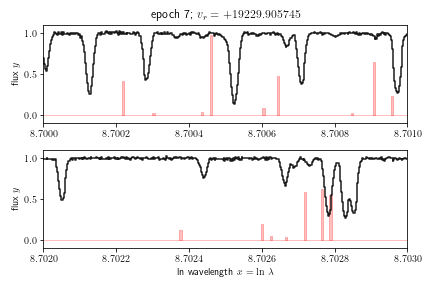
\includegraphics[width=\textwidth]{../notebook/binarymask.png}
    \end{center}
    \caption{A visualization of part of the binary mask. The dark black step function shows the same spectral segment shown in \figref{fig:datazoom}, but the light red filled step function shows the binary mask employed in the text, Doppler shifted to the correct Doppler shift for this epoch. Note that the binary mask is zeroed out in a segment at the left edge of the top plot; this is a result of the censoring of lines that might Doppler shift in and out of the observed spectral range.\label{fig:binarymask}}
  \end{mdframed}
\end{figure}

\figref{fig:bccfrvswrong} shows that the cross-correlations of the binary mask with the toy spectral data by themselves deliver radial-velocity estimates that don't come close to saturating the information-theoretic bound.
That's not surprising; the maximum-likelihood and cross-correlation radial-velocity estimates are only efficient when the spectral template is an accurate representation of the spectral expectation.
However, \figref{fig:bccfrvs} shows how the radial-velocity estimates improve when the binary-mask cross-correlation functions are subsequently fit with a Gaussian that looks like the line-spread function.
These post-processed binary-mask results do saturate the bound.

\begin{figure}[tp]
  \begin{mdframed}
    \begin{center}
    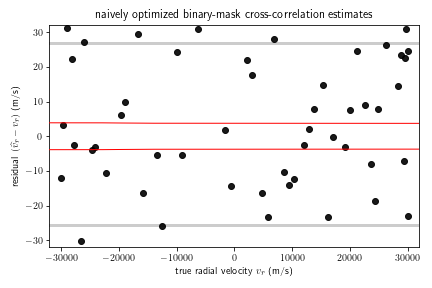
\includegraphics[width=\textwidth]{../notebook/bccfrvswrong.png}
    \end{center}
    \caption{Same as the bottom panel of \figref{fig:mlrvs} but showing the results of naively optimizing the cross-correlation of the data with the binary mask. These estimates do not saturate the information-theoretic bound because the binary mask is not a good representation of the spectral expectation.\label{fig:bccfrvswrong}}
  \end{mdframed}
\end{figure}%
\begin{figure}[tp]
  \begin{mdframed}
    \begin{center}
    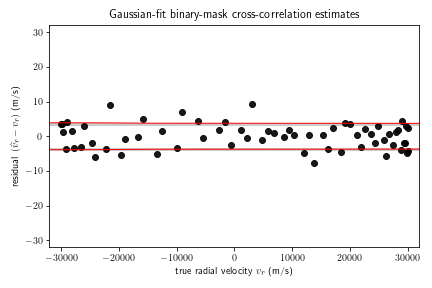
\includegraphics[width=\textwidth]{../notebook/bccfrvs.png}
    \end{center}
    \caption{Same as the bottom panel of \figref{fig:mlrvs} but showing the results of optimizing the fit of a Gaussian function to the cross-correlation of the data with the binary mask. Compare this with \figref{fig:bccfrvswrong}. Binary-mask cross-correlation functions deliver bound-saturating Doppler-shift estimates when fit after the fact with a Gaussian function. See text for discussion.\label{fig:bccfrvs}}
  \end{mdframed}
\end{figure}

Experiments suggest that the binary-mask operations are very sensitive to edge effects.
In making the mask, we removed lines near the edges of the observed spectral range, so that our results aren't contaminated by variations resulting from lines entering and leaving the spectral range.
This probably leads to a small loss in precision, but the results saturate the information-theoretic bound nonetheless.

\section{Empirical spectral templates}\label{sec:templates}

The most important thing about radial-velocity variations with time---for a star with a constant intrinsic spectrum---is that the variations can be measured empirically, without any fundamental physical beliefs about the star (other than its lack of intrinsic variability).
That is, the investigator does not need to approach the problem with a good-fitting theoretical stellar spectral template $f(x)$.
The spectral template $f(x)$ can be derived directly from the observations of the star themselves.
The requirement here is that there be substantial numbers of epochs of observations, sufficient to provide an estimate of the mean spectrum that is (much) higher in signal-to-noise than the spectral data at any individual epoch.
This realization is the fundamental motivation for the \wobble{} project (\citealt{wobble}).

HOGG: Quantitative argument using SNR and scalings.

Empirical templates can be created by interpolating spectra to a common logarithmic wavelength grid and averaging.
Interpolations wwre performed with cubic splines.
With an empirical template in hand, cross-correlation doppler shifts can be estimated, updating the beliefs about the spectra rest frames, and then the templates can be re-made.
This process can be iterated to convergence.
In this process, the initialization matters.
In making the results in this \sectionname, we initialized at the wrong binary-mask results shown in \figref{fig:bccfrvswrong}, not at good radial-velocities, and yet the results are excellent.
That is, we didn't cheat.
We show the empirical template in \figref{fig:empirical} and we show the
empirical-spectrum cross-correlation radial-velocity results in \figref{fig:empiricalrvs}

\begin{figure}[tp]
  \begin{mdframed}
    \begin{center}
    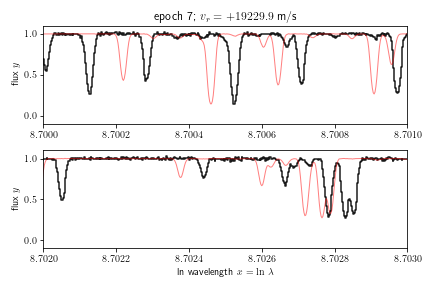
\includegraphics[width=\textwidth]{../notebook/empirical.png}
    \end{center}
    \caption{A visualization of part of the empirical spectral template. The dark black step function shows the same spectral segment shown in \figref{fig:datazoom}, but the thin red smooth line now shows not the true spectral template but instead the empirical template obtained by shifting and averaging the observed data. Note that the empirical template constructed here has no lines in a segment at the left edge of the top plot; this is a result of the censoring of spectral regions that might Doppler shift in and out of the observed spectral range.\label{fig:empirical}}
  \end{mdframed}
\end{figure}
\begin{figure}[tp]
  \begin{mdframed}
    \begin{center}
    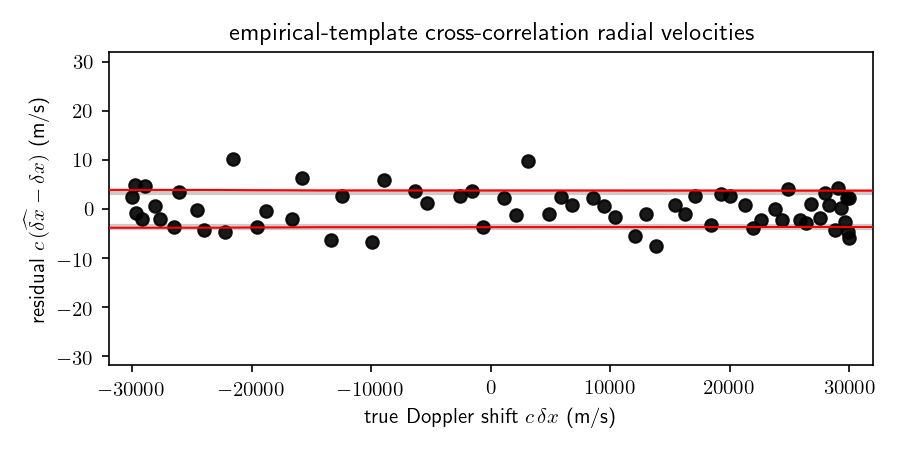
\includegraphics[width=\textwidth]{../notebook/empiricalrvs.png}
    \end{center}
    \caption{Same as the bottom panel of \figref{fig:mlrvs} but showing the results of optimizing the cross-correlation of the data with an empirical template made from the epoch data themselves. Compare with \figref{fig:ccfrvs}; this shows that empirical templates are just as good as true templates; they both saturate the information-theoretic bounds.\label{fig:empiricalrvs}}
  \end{mdframed}
\end{figure}

HOGG: Note the sensitivity to edge effects.... How did we deal with that?

HOGG: IS THERE A BIAS WHEN YOU USE THE SPECTRUM IN ITS OWN ANALYSIS? EXPERIMENT WITH LOO. (Later: Did this; it is a very small effect at this sample size. Maybe try a smaller sample?)

HOGG: Note that there is no absolute velocity here.

\section{Sensitivity to assumptions}\label{sec:sensitivity}

We opened (\secref{sec:assumptions}) with a long list of restrictive assumptions.
Here we perform experiments in which we make the data weakly incompatible with some of these assumptions and look at how the radial-velocity measurements are affected.

\noindent
\paragraph{Wavelength calibration issues}
In \secref{sec:assumptions} and everything else above, we assumed that...HOGG

\begin{figure}[tp]
  \begin{mdframed}
    \begin{center}
    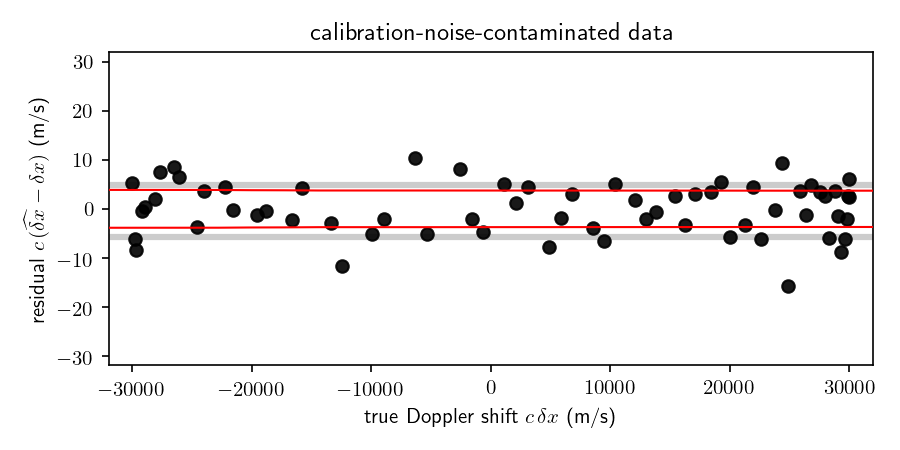
\includegraphics[width=\textwidth]{../notebook/calibration.png}
    \end{center}
    \caption{Same as \figref{fig:ccfrvs} but now showing cross-correlation results after systematic wavelength-calibration issues are introduced. THe calibration issues are below the one-thousandth-of-a-pixel level and have no net Doppler shift (see text).\label{fig:calibration}}
  \end{mdframed}
\end{figure}

\noindent
\paragraph{Unmodeled low-amplitude telluric lines}
In \secref{sec:assumptions} and everything else above, we assumed that telluric lines either don't exist, or else are handled properly.
Telluric lines can be handled by fitting and subtracting them, or by masking the data at their locations.
However, it is possible for there to be tiny, unknown telluric features that affect the data but aren't either known or individually detectable.
(HOGG COMMENT that wobble can handle these!)
Here we test the sensitivity to this assumption by adding in HOGG WHAT AND HOW?

\begin{figure}[tp]
  \begin{mdframed}
    \begin{center}
    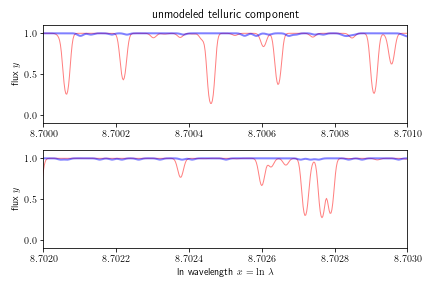
\includegraphics[width=\textwidth]{../notebook/telluricmodel.png}
    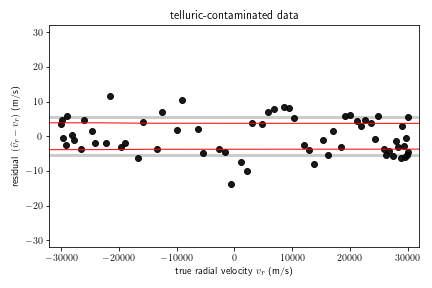
\includegraphics[width=\textwidth]{../notebook/telluric.png}
    \end{center}
    \caption{The top panels show the introduced telluric effect in blue, in comparison with the true spectral template (in red, repeated from \figref{fig:datazoom}). The bottom panel is the same \figref{fig:ccfrvs} but now showing cross-correlation results after this unmodeled telluric contamination is introduced.\label{fig:variable}}
  \end{mdframed}
\end{figure}

\noindent
\paragraph{Small spectral variations}
In \secref{sec:assumptions} and everything else above, we assumed that...HOGG

\begin{figure}[tp]
  \begin{mdframed}
    \begin{center}
    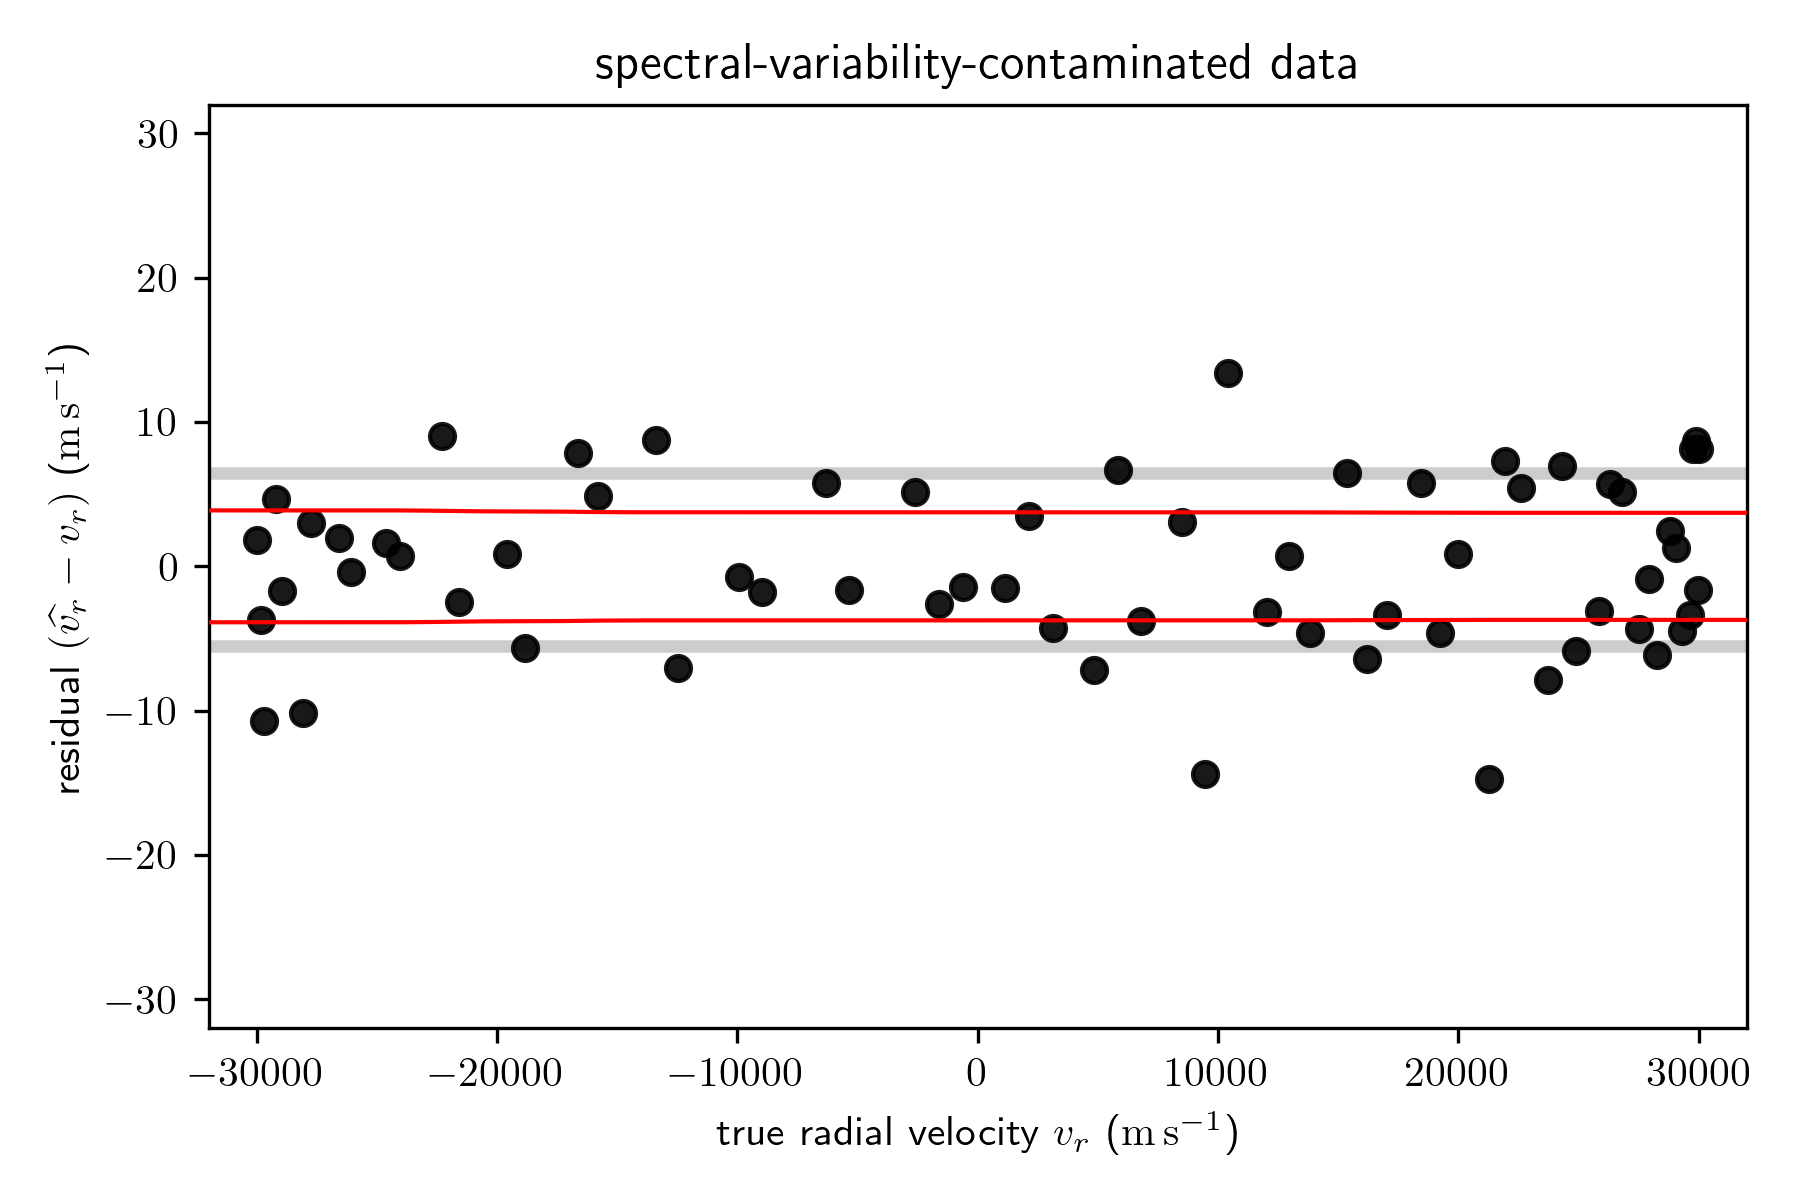
\includegraphics[width=\textwidth]{../notebook/variable.png}
    \end{center}
    \caption{Same as \figref{fig:ccfrvs} but now showing cross-correlation results after spectral variability is introduced. The variability is at the percent level in equivalent widths, only in the line equivalent widths, and not at all in line locations (see text).\label{fig:variable}}
  \end{mdframed}
\end{figure}

\section{Discussion}\label{sec:discussion}

HOGG: Return to the assumptions and discuss them at least briefly, and what happens if you want to weaken them.

HOGG: In the above, make sure to comment on the conceptual point of whether you are measuring a velocity wrt the spectrograph, or a velocity wrt the Solar-System barycenter (as EXPRES does). This distinction is important to the design of extraction pipelines, but doesn't change any of our story here.

HOGG: Do the time-invariant spectrum assumption last and discuss the different possible approaches to this problem.

\software{
\project{numpy} \citep{numpy};
\project{matplotlib} \citep{matplotlib}
\project{scipy} \citep{scipy}
}

\begin{acknowledgments}
It is a pleasure to thank
  Jacob Bean (Chicago),
  John Brewer (Yale),
  Dan Foreman-Mackey (Flatiron),
  Ben Montet (Chicago),
  Adrian Price-Whelan (Flatiron),
  Hans-Walter Rix (MPIA),
  Julian Stuermer (Chicago),
  Lily Zhao (Flatiron),
and the Astronomical Data Group at the Flatiron Institute for valuable discussions and input.
MB thanks the Max-Planck-Institut f\"ur Astronomie in Heidelberg
for hospitality during a critical phase of this project.
\end{acknowledgments}

\begin{thebibliography}{dummy}
  \bibitem[Bedell et al.(2019)]{wobble} Bedell, M., Hogg, D.~W., Foreman-Mackey, D., et al.\ 2019, \aj, 158, 164. doi:10.3847/1538-3881/ab40a7
  \bibitem[Blackman et al.(2019)]{berv-lambda} Blackman, R.~T., Ong, J.~M.~J., \& Fischer, D.~A.\ 2019, \aj, 158, 40. doi:10.3847/1538-3881/ab24c3
  \bibitem[Harris et al.(2020)]{numpy} Harris, C.~R., Millman, K.~J., van der Walt, S.~J., et al.\ 2020, \nat, 585, 357. doi:10.1038/s41586-020-2649-2
  \bibitem[Hubble(1929)]{hubble} Hubble, E.\ 1929, Proceedings of the National Academy of Science, 15, 168. doi:10.1073/pnas.15.3.168
  \bibitem[Hunter(2007)]{matplotlib} Hunter, J.~D.\ 2007, Computing in Science and Engineering, 9, 90. doi:10.1109/MCSE.2007.55
  \bibitem[Mayor \& Queloz(1995)]{mayor} Mayor, M. \& Queloz, D.\ 1995, \nat, 378, 355. doi:10.1038/378355a0
  \bibitem[Rubin et al.(1980)]{rubin} Rubin, V.~C., Ford, W.~K., \& Thonnard, N.\ 1980, \apj, 238, 471. doi:10.1086/158003
  \bibitem[Virtanen et al.(2020)]{scipy} Virtanen, P., Gommers, R., Oliphant, T.~E., et al.\ 2020, Nature Methods, 17, 261. doi:10.1038/s41592-019-0686-2
  \bibitem[Zhao(2021)]{zhaophd} Zhao, L.~L., 2021, PhD dissertation, Yale University
  \bibitem[Zwicky(1933)]{zwicky} Zwicky, F.\ 1933, Helvetica Physica Acta, 6, 110
\end{thebibliography}

\end{document}
